%%%%%%%%%%%%%%%%%%%%%%%%%%%%%%%%%%%%%%%%%%%%%%%%%%%%%%%%%%%%%%%%%%%%%
% LaTeX Template: Project Titlepage Modified (v 0.1) by rcx
%
% Original Source: http://www.howtotex.com
% Date: February 2014
% 
% This is a title page template which be used for articles & reports.
% 
% This is the modified version of the original Latex template from
% aforementioned website.
% 
%%%%%%%%%%%%%%%%%%%%%%%%%%%%%%%%%%%%%%%%%%%%%%%%%%%%%%%%%%%%%%%%%%%%%%

%-------------------------------------------------------------------------------
% TITLE PAGE
%-------------------------------------------------------------------------------

\documentclass[12pt]{report}
\usepackage[a4paper]{geometry}
\usepackage[myheadings]{fullpage}
\usepackage{fancyhdr}
\usepackage{lastpage}
\usepackage{graphicx, wrapfig, subcaption, setspace, booktabs}
\usepackage[T1]{fontenc}
\usepackage[font=small, labelfont=bf]{caption}
\usepackage{fourier}
\usepackage[protrusion=true, expansion=true]{microtype}
\usepackage[english]{babel}
\usepackage{biblatex}
\bibliography{references}
\usepackage{sectsty}
\usepackage{url, lipsum}
\usepackage{listings}
\usepackage{color}

\definecolor{mygray}{rgb}{0.9,0.9,0.9}

\lstset{
    backgroundcolor=\color{mygray}
}

\newcommand{\HRule}[1]{\rule{\linewidth}{#1}}
\onehalfspacing
\setcounter{tocdepth}{5}
\setcounter{secnumdepth}{5}

%-------------------------------------------------------------------------------
% HEADER & FOOTER
%-------------------------------------------------------------------------------
\pagestyle{fancy}
\fancyhf{}
\setlength\headheight{15pt}
\fancyhead[L]{Administración de Redes y Seguridad - 2018}
\fancyhead[R]{Toledo Margalef}
\fancyfoot[R]{Page \thepage\ of \pageref{LastPage}}


\begin{document}

\title{ \normalsize \textsc{Administración de Redes y Seguridad}
        \\ [2.0cm]
        \HRule{0.5pt} \\
        \LARGE \textbf{\uppercase{Trabajo Práctico 4}}
        \HRule{2pt} \\ [0.5cm]
        \normalsize \today \vspace*{5\baselineskip}}

\date{}

\author{
        Cátedra: \\
        Lic: Zappellini, Bruno Damian \\
\\
        Integrantes: \\
        Toledo Margalef, Pablo Adrian \\
        UNPSJB - Trelew}

\maketitle


\tableofcontents
\newpage

%-------------------------------------------------------------------------------
% Section title formatting
\sectionfont{\scshape}
%-------------------------------------------------------------------------------

%-------------------------------------------------------------------------------
% BODY
%-------------------------------------------------------------------------------

\section*{1. Footprinting}
\addcontentsline{toc}{section}{Footprinting}

\subsection*{¿Qué es footprinting?}

Footprinting \nocite{WikipediaFootprinting}, también conocido como \texttt{reconocimiento} es una técnica utilizada para recolectar información sobre dispositivos y su entorno. Dentro de los métodos que se pueden utilizar se encuentran:

\begin{itemize}
    \item Consultas DNS
    \item Identificación de sistema Operativo (nmap)
    \item Escaneo de puertos
    \item Querys de WHOIS
    \item google hacking
\end{itemize}

\subsubsection*{DIG y WHOIS}

Se utilizaran las siguientes dos organizaciones

\begin{itemize}
    \item Administración Federal de Ingresos Públicos
        \begin{itemize}
            \item \texttt{afip.gov.ar}
        \end{itemize}
    \item IBM
        \begin{itemize}
            \item \texttt{ibm.com} 
        \end{itemize}
\end{itemize}

\textbf{DIG}: es una herramienta para realizar peticiones a servidores de nombres. tomando un nombre de dominio y realizando el lookup correspondiente.

\textbf{WHOIS}: herramienta que busca un nombre de dominio en la base de datos de ls RFC 3912, la base de datos que almacena la correspondencia entre usuarios registrados y nombres de dominio.

Realizamos las consultas utilizando \texttt{afip.gov.ar} y listamos los resultados

\begin{itemize}
    \item name: ADMINISTRACION FEDERAL DE INGRESOS PUBLICOS
    \item IP (dns lookup): 200.1.116.6
    \item Fecha de registro:  1997-05-26 00:00:00
    \item Fecha expiración: 2019-06-25 00:00:00
    \item Servidor de nombres: ns1.afip.gov.ar (200.1.116.10/32)
    \item Registrar: nicar
\end{itemize}

Ahora con \texttt{ibm.com} 

\begin{itemize}
    \item name: IBM.COM
    \item IP (dns lookup): 129.42.38.10
    \item Fecha de registro: 1986-03-19T05:00:00Z
    \item Fecha expiración: 2019-03-20T04:00:00Z
    \item Servidor de nombres: EUR2.AKAM.NET
    \item Registrar: CSC Corporate Domains, Inc.
\end{itemize}

\subsection*{NETCRAFT - www.unp.edu.ar}

Realizamos la consulta en \texttt{netcraft.net} sobre \texttt{www.unp.edu.ar} y listamos algunos datos que se muestran allí.

\begin{tabular}{l | l}
    \hline 
    Site title & Universidad Nacional de la Patagonia San Juan Bosco \\ \hline
    Date first seen & June 1998 \\ \hline
    language & Spanish \\ \hline
    Description & Sitio web de la Universidad Nacional de la Patagonia San Juan Bosco. \\ \hline
    Netcraft Risk Rating & 7/10 \\ \hline
    Netblock Owner & Red de Interconexion Universitaria \\ \hline
    Nameserver & chenque.unp.edu.ar \\ \hline
    IP address & 170.210.88.21 (VirusTotal) \\ \hline
    DNS admin & hostmaster@unp.edu.ar \\ \hline
    Hosting company & unp.edu.ar \\ \hline
    Top Level Domain & Argentina (.edu.ar) \\ \hline
    Hosting country & AR \\ \hline
    
\end{tabular}

\subsection*{archive.org}

Este sitio ofrece, una snapshot del sitio que se busque. Proviendo las cualidades, casi, completas que nos ofrecía. De este modo, si en algún momento se dejó al descubierto alguna información de valor y se realizó la snapshot, ese dato está disponible, por más que se haya cambiado en el sitio real.

\subsection*{Fingerprinting}

\begin{itemize}
    \item \textbf{www.google.com.ar}: gws ()
    \item \textbf{www.ing.unp.edu.ar}: nginx/1.10.3
    \item \textbf{www.microsoft.com}: Apache
    \item \textbf{www.google.com.ar}: Microsoft-IIS/10.0
\end{itemize}

\section*{Sección 2}

\subsection*{Scanning}

Consiste en la búsqueda exhaustiva de diversas cuestiones a determinado nivel o niveles para encontrar vulnerabilidades.

El \textbf{escaneo de hosts} se realiza dentro una subred y permite enumerar los dispositivos que se encuentran conectados a ella. Teniendo como objetivo un equipo en particular, se puede realizar un \textbf{escaneo de puertos} de forma tal que se puede saber qué puertos se encuentran abiertos y disponibles para inciar una conexión.

Cuando se cuenta con red de Wi-Fi se puede realizar un \textbf{escaneo de redes Wi-Fi} para identificar las redes disponibles y poder hacer algún ataque a alguna en particular. Lo mismo se puede hacer cuando se tiene conectividad por bluetooh, listando los dispositivos disponibles para atacar.


\subsection*{Posibilidad de escaneo}

\begin{itemize}
    \item Sólo manipulando ARP: Escaneo de Hosts. Requiere estar en el mismo segmento de red.
    \item Sólo manipulando ICMP: Escaneo de puertos y host. No requiere estar en la misma red.
    \item Sólo manipulando TCP: Escaneo de puertos. No requiere estar en la misma red.
    \item Sólo manipulando UDP: Escaneo de puertos. No requiere estar en la misma red
    \item Interpretando tráfico: Escaneo de Wi-Fi, Bluetooth. Hosts y puertos. Se puede estar fuera de la red, en el caso de las radiofrecuencias. Salvo para LAN, ahí es mandatorio estar dentro de alguna red. 
\end{itemize}

\subsection*{Escaneo de puertos}

En la máquina virtual provsita por la cátedra, como primera medida, ponemos a funcionar el servicio de ssh, que atiende en el puerto 22 y corremos el comando netstat para verificar la existencia de puertos abiertos.

\begingroup
    \fontsize{8pt}{10pt}\selectfont
\begin{lstlisting}[breaklines=true]
root@kali:~# netstat -nltp4
Active Internet connections (only servers)
Proto Recv-Q Send-Q Local Address           Foreign Address         State       PID/Program name    
tcp        0      0 0.0.0.0:22              0.0.0.0:*               LISTEN      1645/sshd           
\end{lstlisting}
\endgroup

Luego, utilizando \texttt{nmap} escaneamos por puertos TCP que se encuentren abiertos.

\begingroup
    \fontsize{9pt}{10pt}\selectfont
\begin{lstlisting}[breaklines=true]
root@kali:~# nmap -sV localhost

Starting Nmap 7.40 ( https://nmap.org ) at 2018-10-15 18:22 EDT
Nmap scan report for localhost (127.0.0.1)
Host is up (0.0000020s latency).
Other addresses for localhost (not scanned): ::1
Not shown: 999 closed ports
PORT   STATE SERVICE VERSION
22/tcp open  ssh     OpenSSH 7.4p1 Debian 10 (protocol 2.0)
Service Info: OS: Linux; CPE: cpe:/o:linux:linux_kernel

Service detection performed. Please report any incorrect results at https://nmap.org/submit/ .
Nmap done: 1 IP address (1 host up) scanned in 0.36 seconds
\end{lstlisting}
\endgroup

Como se puede observar, el puerto 22 (propio de ssh) fue detectado por nmap.

\pagebreak

Seguidamente, le pedimos a \texttt{nmap}, explicitamente, que escanee los 65536 puertos disponibles.

\begingroup
    \fontsize{9pt}{10pt}\selectfont
\begin{lstlisting}[breaklines=true]
root@kali:~# nmap -p0-65535 localhost

Starting Nmap 7.40 ( https://nmap.org ) at 2018-10-15 18:52 EDT
Nmap scan report for localhost (127.0.0.1)
Host is up (0.0000020s latency).
Other addresses for localhost (not scanned): ::1
Not shown: 65535 closed ports
PORT   STATE SERVICE
22/tcp open  ssh

Nmap done: 1 IP address (1 host up) scanned in 0.57 seconds
\end{lstlisting}
\endgroup

\subsubsection*{Escaneo manual de puertos}

\textbf{hping3 -c 3 -S -p 80 localhost}: en la salida del analizador de protocolos se observa que el host responde con la bandera de \texttt{reset}. Indicando que el puerto está cerrado. En este caso se realiza un escaneo de tipo SYN. Ya que sólo se envía un paquete con la bandera \texttt{SYN}, imitando el inicio de una conexión.


\textbf{hping3 -c 3 -S -p 113 localhost}: en la salida del analizador de protocolos observamos un comportamiento similar al del inciso anterior. El puerto se encuentra cerrado y por lo tanto responde con la bandera de \texttt{reset} en 1


\textbf{hping3 -c 3 -2 127.0.0.1 -p 631}: se observa que el puerto 631, usado para \texttt{internet printing} se encuentra cerrado. En este caso, el método de escaneo de puertos utilizado, debido a que UDP es un protocolo carente de estado consiste en el envío de un paquete ICMP, considerando la respuesta de un \texttt{icmp port unreachable} como que el puerto se encuentra cerrado. Si el puerto no responde se considera abierto, lo cual no sucede en este caso.

\textbf{hping3 -c 3 -2 127.0.0.1 -p 53}: como con el inciso anterior el puerto responde con un \texttt{icmp port unreachable}, indicando que el puerto se encuentra cerrado.


\subsubsection*{IDLE Scan}

Para la realización de IDLE scan el equipo a utilizar como zombie debe tener poco tráfico e IPID predecibles.

\section*{Fingerprinting}

El Fingerprinting es una técnica de recolección de información de un equipo para su identificación. Dentro de las cualidades de las que se pueden hacen fingerprinting se encuentra el Sistema Operativo. Descubrir el Sistema Operativo, en especial su versión, de un equipo puede servir para saber qué posibles fallas de seguridad posee y sus formas de explotarlas.

En mi maquina local, dentro de la red de mi casa, levanto la máquina virtual provista por la cátedra, una segunda máquina virtual con Windows 7 y corre el comando

\begingroup
    \fontsize{9pt}{10pt}\selectfont
\begin{lstlisting}[breaklines=true]
Starting Nmap 7.70 ( https://nmap.org ) at 2018-10-24 01:31 -03
Nmap scan report for 192.168.0.1
Host is up (0.0034s latency).
Not shown: 955 filtered ports, 44 closed ports
PORT   STATE SERVICE
80/tcp open  http
MAC Address: 00:21:27:E7:81:04 (Tp-link Technologies)
Device type: media device|broadband router|general purpose
Running: VBrick embedded, Westell embedded, Wind River VxWorks
OS CPE: cpe:/h:vbrick:4300 cpe:/h:westell:wirespeed_6100 cpe:/o:windriver:vxworks
OS details: VBrick 4300 video encoder, Westell WireSpeed Dual Connect 6100 DSL router, VxWorks
Network Distance: 1 hop

Nmap scan report for 192.168.0.101
Host is up (0.00064s latency).
All 1000 scanned ports on 192.168.0.101 are closed
MAC Address: 08:00:27:A1:B6:E6 (Oracle VirtualBox virtual NIC)
Too many fingerprints match this host to give specific OS details
Network Distance: 1 hop

Nmap scan report for 192.168.0.102
Host is up (0.00058s latency).
Not shown: 999 filtered ports
PORT     STATE SERVICE
5357/tcp open  wsdapi
MAC Address: 08:00:27:10:26:4E (Oracle VirtualBox virtual NIC)
Warning: OSScan results may be unreliable because we could not find at least 1 open and 1 closed port
Device type: general purpose|phone
Running: Microsoft Windows 2008|8.1|7|Phone|Vista
OS CPE: cpe:/o:microsoft:windows_server_2008::beta3 cpe:/o:microsoft:windows_server_2008 cpe:/o:microsoft:windows_8.1 cpe:/o:microsoft:windows_7::-:professional cpe:/o:microsoft:windows_8 cpe:/o:microsoft:windows cpe:/o:microsoft:windows_vista::- cpe:/o:microsoft:windows_vista::sp1
OS details: Microsoft Windows Server 2008 or 2008 Beta 3, Microsoft Windows Server 2008 R2 or Windows 8.1, Microsoft Windows 7 Professional or Windows 8, Microsoft Windows 8.1 R1, Microsoft Windows Phone 7.5 or 8.0, Microsoft Windows Vista SP0 or SP1, Windows Server 2008 SP1, or Windows 7, Microsoft Windows Vista SP2, Windows 7 SP1, or Windows Server 2008
Network Distance: 1 hop

Nmap scan report for 192.168.0.103
Host is up (0.00013s latency).
Not shown: 998 closed ports
PORT     STATE SERVICE
22/tcp   open  ssh
5432/tcp open  postgresql
Device type: general purpose
Running: Linux 3.X
OS CPE: cpe:/o:linux:linux_kernel:3
OS details: Linux 3.7 - 3.10
Network Distance: 0 hops

OS detection performed. Please report any incorrect results at https://nmap.org/submit/ .
Nmap done: 256 IP addresses (4 hosts up) scanned in 19.26 seconds
    
\end{lstlisting}
\endgroup

Vemos que responde correctamente en el caso de las máquinas virtual, pero al llegar a la máquina virtual vemos que indica que \texttt{Too many fingerprints match this host to give specific OS details}, dando a entender que la información que recabó del host no le permitió dar con una cantidad reducida de identidades para asignarle.

Otra versión de este tipo de fingerprinting es la de realizarlo con servicios, en lugar del Sistema Operativo. Debido a que un servicio también sirve de puerta de entrada a un equipo a través de la red, creería que en ocasiones siendo una oportunidad más posible de llevar adelante. Este tipo de fingerprint se puede realizar a través de banner grabbing, pero no es la única forma, podemos realizar un ping sweeping a lo largo de puertos bien conocidos que querramos inspeccionar en caso de encontrar un servicio que podamos usar de puerta de entrada.

\section*{Enumeración}

La \textbf{enumaración} es una técnica por la cual se obtiene un listado de usuarios, dispositivos o hosts presentes en una red. Este procedimiento se puede realizar de diversas maneras, dependiendo del medio físico utilizado en la red.

\begin{itemize}
    \item Wifi: para enumerar las redes wifi presentes en la facultad bastaría con realizar una consulta al adaptador de red, para que provea el SSID e intensidad de cada red que está detectando. También nos interesa saber el nivel de seguridad que poseen.
    \item Bluetooth: Utilizando el adaptador podemos saber la cantidad y qué dispositivos Bluetooth se encuentran presentes en la red.
    \item Recursos presentes en una red windows: Dentro de una red de windwos, la enumeración se puede realizar, primero habilitando la detección de redes y de recursos compartidos de nuestro equipo y luego en la pestaña de red del explorador se mostaran los distitos recursos alcanzables por nuestro equipo.
    \item Información de DNS de algún dominio en particular: Realizando consultas bien dirigidad al servidor. Esta técnica considero que puede ser fácilmente detectable como maliciosa, ya que al realizar algunas consultas en cierto orden se vuelve casi aparente que el usuario no es bien intencionado.
\end{itemize}

Al intentar realizar una enumeración DNS utilizando el dominio \texttt{unp.edu.ar} nos devuelve error, pero al intentarlo con \texttt{google.com} obtenemos lo especificado en el archivo \texttt{salida-dns-enum.xml} adjunto con el informe.

\section*{Ataques de fuerza bruta}

Demostramos un ataque por fuerza bruta sobre ssh en la máquina virtual provista por la cátedra

\begingroup
    \fontsize{8pt}{10pt}\selectfont
\begin{lstlisting}[breaklines=true]
msf > use auxiliary/scanner/
Display all 540 possibilities? (y or n)
msf > use auxiliary/scanner/ssh/ssh_login
msf auxiliary(scanner/ssh/ssh_login) > set rhosts 192.168.0.101
rhosts => 192.168.0.101
msf auxiliary(scanner/ssh/ssh_login) > set pass_file /home/pablo/shared/badpasswords
pass_file => /home/pablo/shared/badpasswords
msf auxiliary(scanner/ssh/ssh_login) > set username defo
username => defo
msf auxiliary(scanner/ssh/ssh_login) > set stop_on_success true
stop_on_success => true
msf auxiliary(scanner/ssh/ssh_login) > exploit

[+] 192.168.0.101:22 - Success: 'defo:defo1234' 'uid=1001(defo) gid=1001(defo) groups=1001(defo) Linux kali 4.9.0-kali3-amd64 #1 SMP Debian 4.9.18-1kali1 (2017-04-04) x86_64 GNU/Linux '
[*] Command shell session 1 opened (192.168.0.103:45081 -> 192.168.0.101:22) at 2018-10-24 03:03:14 -0300
[*] Scanned 1 of 1 hosts (100% complete)
[*] Auxiliary module execution completed
msf auxiliary(scanner/ssh/ssh_login) > sessions

Active sessions
===============

  Id  Name  Type         Information                           Connection
  --  ----  ----         -----------                           ----------
  1         shell linux  SSH defo:defo1234 (192.168.0.101:22)  192.168.0.103:45081 -> 192.168.0.101:22 (192.168.0.101)

msf auxiliary(scanner/ssh/ssh_login) > sessions -i 1
[*] Starting interaction with 1...

whoami
defo
uname -a
Linux kali 4.9.0-kali3-amd64 #1 SMP Debian 4.9.18-1kali1 (2017-04-04) x86_64 GNU/Linux
\end{lstlisting}
\endgroup

Utilizando la herramienta \texttt{Hydra-gtk} provista en la máquina virtual podemos realizar el mismo ataque, pero esta vez desde una ventana. La salida que devuelve es la siguiente:

\begingroup
    \fontsize{8pt}{10pt}\selectfont
\begin{lstlisting}[breaklines=true]
Hydra v8.3 (c) 2016 by van Hauser/THC - Please do not use in military or secret service organizations, or for illegal purposes.

Hydra (http://www.thc.org/thc-hydra) starting at 2018-10-24 02:22:12
[DATA] max 16 tasks per 1 server, overall 64 tasks, 21 login tries (l:1/p:21), ~0 tries per task
[DATA] attacking service ssh on port 22
[WARNING] Many SSH configurations limit the number of parallel tasks, it is recommended to reduce the tasks: use -t 4
[22][ssh] host: localhost   login: defo   password: defo1234
1 of 1 target successfully completed, 1 valid password found
Hydra (http://www.thc.org/thc-hydra) finished at 2018-10-24 02:22:14
<finished>
\end{lstlisting}
\endgroup

Vemos que la contraseña encontrada es la correcta y nos permite autenticarnos en la máquina virtual utilizando esas credenciales.

\section*{Sección 3}

\subsection*{Firewall}

\begin{enumerate}
    \item Se utilizó una política restrictiva
    \item No son suficientes las reglas implementadas, pues no se acepta el acceso al equipo que tiene el servidor en el puerto 443, que es el puerto bien conocido para HTTPS.

        Teniendo en cuenta que tampoco se están permitiendo que las conexiones ya establecidas con el puerto 80 se puedan mantener.

        Para poder hacer lo que se está pidiendo deberían implementarse las siguientes reglas, además de las ya implementadas.

\begin{lstlisting}[breaklines=true]
iptables -A FORWARD -p tcp --dport 80 -d 200.10.11.2 -m state --state ESTABLISHED,RELATED -j ACCEPT
iptables -A FORWARD -p tcp --dport 443 -d 200.10.11.2 -j ACCEPT
iptables -A FORWARD -p tcp --dport 443 -m state --state ESTABLISHED,RELATED -j ACCEPT
\end{lstlisting}

De esta forma permite que desde internet se puedan realizar conexiones al servidor web y poder mantenerlas, tanto al puerto 80 como al 443.

Siguiendo con el ejercicio, si además, desde la estación Y se quisiera realizar exitosamente un ping a google, se deberían agregar las siguientes reglas.

\begin{lstlisting}[breaklines=true]
iptables -A FORWARD -p icmp -s 200.10.11.100 -j ACCEPT
iptables -A FORWARD -p icmp -m state --state ESTABLISHED,RELATED -j ACCEPT
\end{lstlisting}

Lo cual permite que las peticiones icmp salientes de Y puedan pasar y luego que circules los paqueted de conexiones ya establecidas bajo el protocolo icmp.
\end{enumerate}

\subsection*{Topología LAN}


Armamos al topología descrita en el enunciado y listamos la configuración de cada nodo

\begingroup
    \fontsize{9pt}{10pt}\selectfont
\begin{lstlisting}[language=bash,breaklines=true]
# Nodo n1
# ifconfig
eth0: flags=4163<UP,BROADCAST,RUNNING,MULTICAST>  mtu 1500
        inet 10.0.0.10  netmask 255.255.255.0  broadcast 10.0.0.255
        inet6 2001::10  prefixlen 64  scopeid 0x0<global>
        inet6 fe80::200:ff:feaa:2  prefixlen 64  scopeid 0x20<link>
        ether 00:00:00:aa:00:02  txqueuelen 1000  (Ethernet)
        RX packets 26  bytes 2124 (2.1 KB)
        RX errors 0  dropped 0  overruns 0  frame 0
        TX packets 13  bytes 1102 (1.1 KB)
        TX errors 0  dropped 0 overruns 0  carrier 0  collisions 0

# netstat -nr
Kernel IP routing table
Destination     Gateway         Genmask         Flags   MSS Window  irtt Iface
0.0.0.0         10.0.0.1        0.0.0.0         UG        0 0          0 eth0
10.0.0.0        0.0.0.0         255.255.255.0   U         0 0          0 eth0

# netstat -natp
# Servicios corriendo por TCP
Active Internet connections (servers and established)
Proto Recv-Q Send-Q Local Address           Foreign Address         State       PID/Program name    
tcp        0      0 0.0.0.0:22              0.0.0.0:*               LISTEN      28/sshd             
tcp6       0      0 :::22                   :::*                    LISTEN      28/sshd  

# netstat -naup
# Servicios corriendo en UDP
Active Internet connections (servers and established)
Proto Recv-Q Send-Q Local Address           Foreign Address         State       PID/Program name

# Nodo n2
# ifconfig 
eth0: flags=4163<UP,BROADCAST,RUNNING,MULTICAST>  mtu 1500
        inet 10.0.0.20  netmask 255.255.255.0  broadcast 10.0.0.255
        inet6 fe80::200:ff:feaa:0  prefixlen 64  scopeid 0x20<link>
        inet6 2001::20  prefixlen 64  scopeid 0x0<global>
        ether 00:00:00:aa:00:00  txqueuelen 1000  (Ethernet)
        RX packets 29  bytes 2414 (2.4 KB)
        RX errors 0  dropped 0  overruns 0  frame 0
        TX packets 14  bytes 1172 (1.1 KB):w
        TX errors 0  dropped 0 overruns 0  carrier 0  collisions 0

# netsat -nr 
Kernel IP routing table
Destination     Gateway         Genmask         Flags   MSS Window  irtt Iface
0.0.0.0         10.0.0.1        0.0.0.0         UG        0 0          0 eth0
10.0.0.0        0.0.0.0         255.255.255.0   U         0 0          0 eth0


# netstat -natp
Active Internet connections (servers and established)
Proto Recv-Q Send-Q Local Address           Foreign Address         State       PID/Program name    

# netstat -naup
Active Internet connections (servers and established)
Proto Recv-Q Send-Q Local Address           Foreign Address         State       PID/Program name

# Nodo n3
# ifconfig 
eth0: flags=4163<UP,BROADCAST,RUNNING,MULTICAST>  mtu 1500
        inet 10.0.0.21  netmask 255.255.255.0  broadcast 10.0.0.255
        inet6 2001::21  prefixlen 64  scopeid 0x0<global>
        inet6 fe80::200:ff:feaa:1  prefixlen 64  scopeid 0x20<link>
        ether 00:00:00:aa:00:01  txqueuelen 1000  (Ethernet)
        RX packets 28  bytes 2304 (2.3 KB)
        RX errors 0  dropped 0  overruns 0  frame 0
        TX packets 15  bytes 1242 (1.2 KB)
        TX errors 0  dropped 0 overruns 0  carrier 0  collisions 0

#netstat -nr
Kernel IP routing table
Destination     Gateway         Genmask         Flags   MSS Window  irtt Iface
0.0.0.0         10.0.0.1        0.0.0.0         UG        0 0          0 eth0
10.0.0.0        0.0.0.0         255.255.255.0   U         0 0          0 eth0

# netstat -natp
Active Internet connections (servers and established)
Proto Recv-Q Send-Q Local Address           Foreign Address         State       PID/Program name    

# netstat -naup
Active Internet connections (servers and established)
Proto Recv-Q Send-Q Local Address           Foreign Address         State       PID/Program name

\end{lstlisting}
\endgroup

Y al momento de correr por primera vez la topología, sin configuración previa, se observa la siguiente salidad de \texttt{iptables} en el server.

\begingroup
    \fontsize{9pt}{10pt}\selectfont
\begin{lstlisting}
# iptables -nL -v
Chain INPUT (policy ACCEPT 0 packets, 0 bytes)
 pkts bytes target     prot opt in     out     source               destination         

Chain FORWARD (policy ACCEPT 0 packets, 0 bytes)
 pkts bytes target     prot opt in     out     source               destination         

Chain OUTPUT (policy ACCEPT 0 packets, 0 bytes)
 pkts bytes target     prot opt in     out     source               destination         
\end{lstlisting}
\endgroup

\subsubsection*{CASO 1}

\texttt{Configure el firewall del Servidor Web para aceptar solamente conexiones al puerto 80 utilizando una política restrictiva.} 


Para poder simular la existencia de un servidor web (puerto 80) haremos uso del comando ncat, con \\
\texttt{ncat -l -p 80 -s <ip-servidor>} \\
luego configuramos el firewall en el server:

\begin{lstlisting}
# Politica restrictiva
iptables -P INPUT DROP
# Aceptar solamente conexiones entrantes al puerto 80 en tcp
iptables -A INPUT -p tcp --dport 80 -j ACCEPT
\end{lstlisting}

\subsubsection*{CASO 2}

\texttt{Configure el firewall del Servidor Web para aceptar solamente conexiones al puerto 80 utilizando una política permisiva.} 

\begin{lstlisting}
# Politica permisiva
iptables -P INPUT ACCEPT

# Toda conexion que no sea para el puerto 80 debería ser descartada
iptables -A INPUT --match multiport -p tcp --dports 23:65535 -j DROP 
iptables -A INPUT --match multiport -p tcp --dports 0:21 -j DROP 
\end{lstlisting}

\subsubsection*{CASO 3}

\texttt{Configure el firewall del Servidor Web para redireccionar toda petición al
puerto TCP 8080 al puerto TCP 80 del mismo equipo}

\begin{lstlisting}
iptables -t nat -A PREROUTING -p tcp --dport 8080 -j REDIRECT --to-ports 22
\end{lstlisting}

\subsubsection*{CASO 4}

\texttt{Configure el firewall del Cliente de modo que, para cualquiera de los puntos anteriores, el mismo pueda establecer hacia el Servidor cualquier tipo de \\comunicación (siempre y cuando el Servidor se lo permita), pero sin permitir que el Web Server pueda iniciar comunicaciones nuevas hacia él.}

\begin{lstlisting}
# Politica Restrictiva
iptables -P OUTPUT DROP

# Permitir conexiones hacia el servidor web pero no permitir que este
# inicie conexiones con el cliente
iptables -A OUTPUT --dst 10.0.0.10 -j ACCEPT
iptables -A INPUT --src 10.0.0.10 -m state --state NEW -j DROP
\end{lstlisting}

\subsection*{Topología Ruteada}

Armamos la topología planteada en el enunciado (respetando el nombre de cada nodo) y revisamos las configuraciones de red de cada nodo. 

\begingroup
    \fontsize{9pt}{10pt}\selectfont
\begin{lstlisting}

# Nodo n1
eth0: flags=4163<UP,BROADCAST,RUNNING,MULTICAST>  mtu 1500
        inet 10.0.1.10  netmask 255.255.255.0  broadcast 10.0.1.255
        inet6 2001:1::10  prefixlen 64  scopeid 0x0<global>
        inet6 fe80::200:ff:feaa:4  prefixlen 64  scopeid 0x20<link>
        ether 00:00:00:aa:00:04  txqueuelen 1000  (Ethernet)
        RX packets 151  bytes 12643 (12.6 KB)
        RX errors 0  dropped 0  overruns 0  frame 0
        TX packets 48  bytes 4725 (4.7 KB)
        TX errors 0  dropped 0 overruns 0  carrier 0  collisions 0

Active Internet connections (servers and established)
Proto Recv-Q Send-Q Local Address           Foreign Address         State       PID/Program name    
tcp        0      0 0.0.0.0:22              0.0.0.0:*               LISTEN      49/sshd             
tcp6       0      0 :::80                   :::*                    LISTEN      65/apache2          
tcp6       0      0 :::22                   :::*                    LISTEN      49/sshd        
Kernel IP routing table
Destination     Gateway         Genmask         Flags   MSS Window  irtt Iface
0.0.0.0         10.0.1.1        0.0.0.0         UG        0 0          0 eth0
10.0.1.0        0.0.0.0         255.255.255.0   U         0 0          0 eth0

Chain INPUT (policy ACCEPT 3 packets, 285 bytes)
 pkts bytes target     prot opt in     out     source               destination         

Chain FORWARD (policy ACCEPT 0 packets, 0 bytes)
 pkts bytes target     prot opt in     out     source               destination         

Chain OUTPUT (policy ACCEPT 3 packets, 201 bytes)
 pkts bytes target     prot opt in     out     source               destination       

# Nodo n2

eth0: flags=4163<UP,BROADCAST,RUNNING,MULTICAST>  mtu 1500
        inet 10.0.0.21  netmask 255.255.255.0  broadcast 10.0.0.255
        inet6 2001::21  prefixlen 64  scopeid 0x0<global>
        inet6 fe80::200:ff:feaa:1  prefixlen 64  scopeid 0x20<link>
        ether 00:00:00:aa:00:01  txqueuelen 1000  (Ethernet)
        RX packets 163  bytes 15011 (15.0 KB)
        RX errors 0  dropped 0  overruns 0  frame 0
        TX packets 32  bytes 2357 (2.3 KB)
        TX errors 0  dropped 0 overruns 0  carrier 0  collisions 0

Active Internet connections (servers and established)
Proto Recv-Q Send-Q Local Address           Foreign Address         State       PID/Program name 

Kernel IP routing table
Destination     Gateway         Genmask         Flags   MSS Window  irtt Iface
0.0.0.0         10.0.0.1        0.0.0.0         UG        0 0          0 eth0
10.0.0.0        0.0.0.0         255.255.255.0   U         0 0          0 eth0

Chain INPUT (policy ACCEPT 0 packets, 0 bytes)
 pkts bytes target     prot opt in     out     source               destination         

Chain FORWARD (policy ACCEPT 0 packets, 0 bytes)
 pkts bytes target     prot opt in     out     source               destination         

Chain OUTPUT (policy ACCEPT 0 packets, 0 bytes)
 pkts bytes target     prot opt in     out     source               destination 

# Nodo n3

eth0: flags=4163<UP,BROADCAST,RUNNING,MULTICAST>  mtu 1500
        inet 10.0.0.20  netmask 255.255.255.0  broadcast 10.0.0.255
        inet6 2001::20  prefixlen 64  scopeid 0x0<global>
        inet6 fe80::200:ff:feaa:0  prefixlen 64  scopeid 0x20<link>
        ether 00:00:00:aa:00:00  txqueuelen 1000  (Ethernet)
        RX packets 190  bytes 16978 (16.9 KB)
        RX errors 0  dropped 0  overruns 0  frame 0
        TX packets 14  bytes 1172 (1.1 KB)
        TX errors 0  dropped 0 overruns 0  carrier 0  collisions 0

Active Internet connections (servers and established)
Proto Recv-Q Send-Q Local Address           Foreign Address         State       PID/Program name    

Kernel IP routing table
Destination     Gateway         Genmask         Flags   MSS Window  irtt Iface
0.0.0.0         10.0.0.1        0.0.0.0         UG        0 0          0 eth0
10.0.0.0        0.0.0.0         255.255.255.0   U         0 0          0 eth0


Chain INPUT (policy ACCEPT 0 packets, 0 bytes)
 pkts bytes target     prot opt in     out     source               destination         

Chain FORWARD (policy ACCEPT 0 packets, 0 bytes)
 pkts bytes target     prot opt in     out     source               destination         

Chain OUTPUT (policy ACCEPT 0 packets, 0 bytes)
 pkts bytes target     prot opt in     out     source               destination         

# Nodo n5

eth0: flags=4163<UP,BROADCAST,RUNNING,MULTICAST>  mtu 1500
        inet 10.0.0.1  netmask 255.255.255.0  broadcast 10.0.0.255
        inet6 2001::1  prefixlen 64  scopeid 0x0<global>
        inet6 fe80::200:ff:feaa:2  prefixlen 64  scopeid 0x20<link>
        ether 00:00:00:aa:00:02  txqueuelen 1000  (Ethernet)
        RX packets 43  bytes 3199 (3.1 KB)
        RX errors 0  dropped 0  overruns 0  frame 0
        TX packets 164  bytes 15125 (15.1 KB)
        TX errors 0  dropped 0 overruns 0  carrier 0  collisions 0

eth1: flags=4163<UP,BROADCAST,RUNNING,MULTICAST>  mtu 1500
        inet 10.0.1.1  netmask 255.255.255.0  broadcast 10.0.1.255
        inet6 fe80::200:ff:feaa:3  prefixlen 64  scopeid 0x20<link>
        inet6 2001:1::1  prefixlen 64  scopeid 0x0<global>
        ether 00:00:00:aa:00:03  txqueuelen 1000  (Ethernet)
        RX packets 49  bytes 4795 (4.7 KB)
        RX errors 0  dropped 0  overruns 0  frame 0
        TX packets 182  bytes 15273 (15.2 KB)
        TX errors 0  dropped 0 overruns 0  carrier 0  collisions 0

Active Internet connections (servers and established)
Proto Recv-Q Send-Q Local Address           Foreign Address         State       PID/Program name    
tcp        0      0 0.0.0.0:2601            0.0.0.0:*               LISTEN      -                   
tcp        0      0 0.0.0.0:2604            0.0.0.0:*               LISTEN      -                   
tcp        0      0 0.0.0.0:2606            0.0.0.0:*               LISTEN      -                   
tcp6       0      0 :::2601                 :::*                    LISTEN      -                   
tcp6       0      0 :::2604                 :::*                    LISTEN      -                   
tcp6       0      0 :::2606                 :::*                    LISTEN      -  


Kernel IP routing table
Destination     Gateway         Genmask         Flags   MSS Window  irtt Iface
10.0.0.0        0.0.0.0         255.255.255.0   U         0 0          0 eth0
10.0.1.0        0.0.0.0         255.255.255.0   U         0 0          0 eth1

\end{lstlisting}
\endgroup

Luego evidenciamos la conexión de red entre los nodos.

\begin{figure}[!ht]
   \centering
   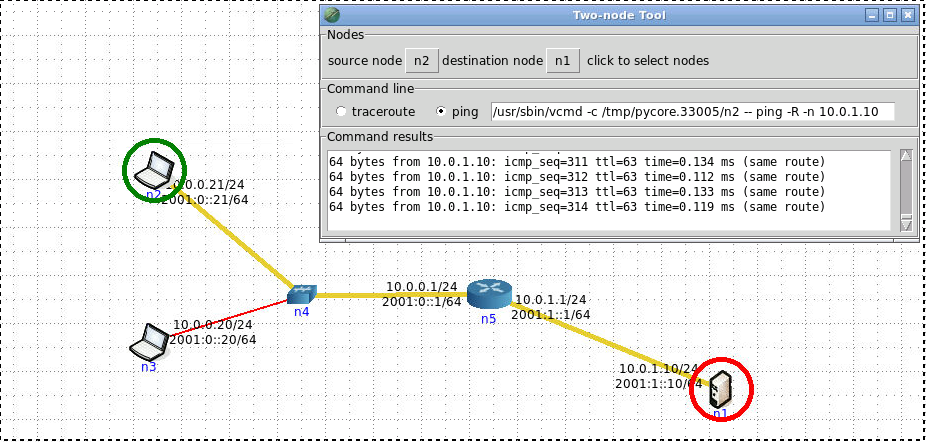
\includegraphics[width=0.9\textwidth]{img/ping-n2-n1}
   \caption{Ping de n2 a n1}
   \centering
   \label{label:file_name}
\end{figure}

\begin{figure}[!ht]
   \centering
   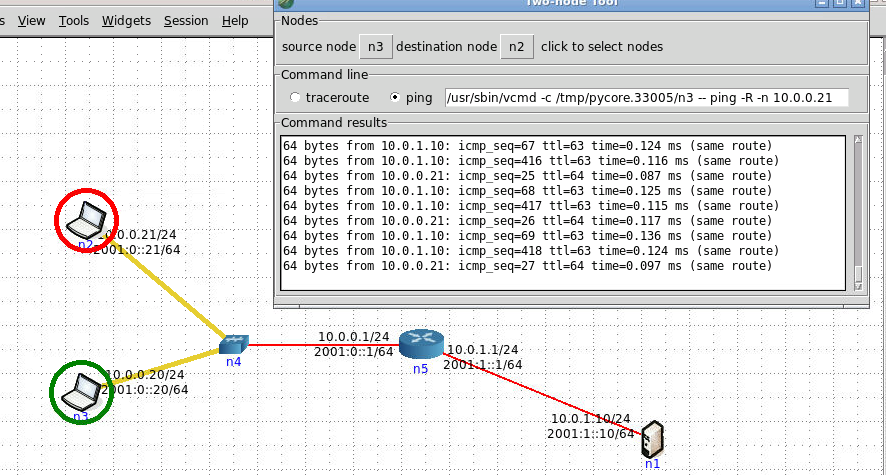
\includegraphics[width=0.9\textwidth]{img/ping-n2-n3}
   \caption{Ping de n2 a n3}
   \centering
   \label{label:file_name}
\end{figure}

\begin{figure}[!ht]
   \centering
   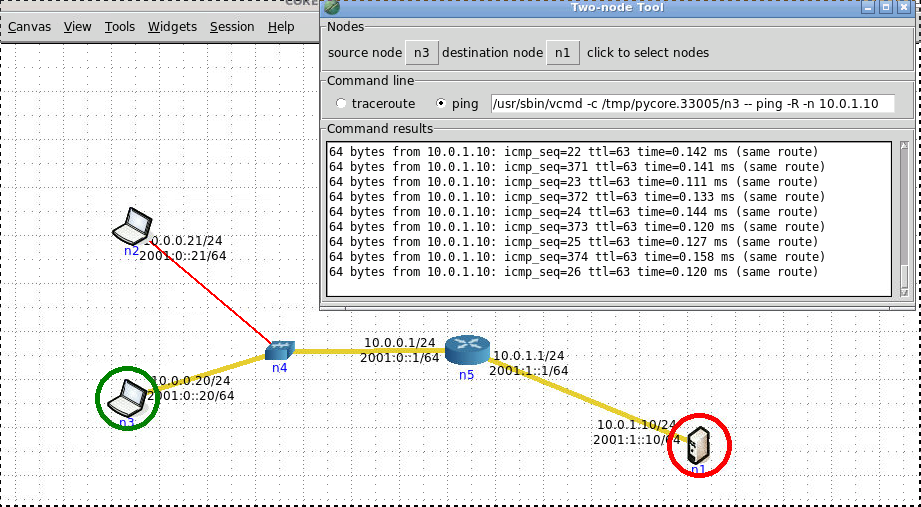
\includegraphics[width=0.9\textwidth]{img/ping-n3-n1}
   \caption{Ping de n3 a n1}
   \centering
   \label{label:file_name}
\end{figure}
\pagebreak

\subsubsection*{Estudio de casos}

Ponemos a correr la topología y luego de correr el script que levante los mock-up de los servicios observamos las siguientes salidas de los comandos \texttt{netstat -nat} y \texttt{netstat -nau}.

\begingroup
    \fontsize{9pt}{10pt}\selectfont
\begin{lstlisting}
# natstat -nat
Active Internet connections (servers and established)
Proto Recv-Q Send-Q Local Address           Foreign Address         State      
tcp        0      0 0.0.0.0:21              0.0.0.0:*               LISTEN     
tcp        0      0 0.0.0.0:22              0.0.0.0:*               LISTEN     
tcp        0      0 0.0.0.0:25              0.0.0.0:*               LISTEN     
tcp        0      0 0.0.0.0:443             0.0.0.0:*               LISTEN     
tcp6       0      0 :::80                   :::*                    LISTEN     
tcp6       0      0 :::22                   :::*                    LISTEN     
tcp6       0      0 :::25                   :::*                    LISTEN     
tcp6       0      0 :::443                  :::*                    LISTEN 

# netstat -nau
Active Internet connections (servers and established)
Proto Recv-Q Send-Q Local Address           Foreign Address         State   
\end{lstlisting}
\endgroup

Listamos las configuraciones del firewall para lograr las siguientes condiciones:

\begingroup
    \fontsize{9pt}{10pt}\selectfont
\begin{lstlisting}
# Se permita únicamente el acceso desde la LAN a los servicios: FTP, SSH y HTTP que corren en el Servidor.

# Borramos las reglas existentes
iptables -F
iptables -X
# Politica Restrictiva
iptables -P FORWARD DROP
# Conexión al servidor en servicio web
iptables -A FORWARD -p tcp --dport 80 --src 10.0.0.0/24 --dst 10.0.1.10 -j ACCEPT
# FTP
iptables -A FORWARD -p tcp --dport 21 --src 10.0.0.0/24 --dst 10.0.1.10 -j ACCEPT
# ssh
iptables -A FORWARD -p tcp --dport 22 --src 10.0.0.0/24 --dst 10.0.1.10 -j ACCEPT
# Dejar pasar en ambos sentidos conexiones ya establecidas y paquetes relacionados
iptables -A FORWARD -m conntrack --ctstate ESTABLISHED,RELATED -j ACCEPT

# Prohibir toda conexión hacia el firewall tanto desde el servidor como desde la LAN
iptables -P INPUT DROP  

# Que desde el Firewall se puedan establecer conexiones SSH hacia el servidor
iptables -A OUTPUT -p tcp --dport 22 --dst 10.0.1.10 -j ACCEPT
iptables -A OUTPUT -p tcp --dport 443 --dst 10.0.1.10 -j ACCEPT
iptables -A INPUT -m state --ctstate ESTABLISHED,RELATED -j ACCEPT

# Permitir conexiones desde el servidor a los clientes de la LAN a través de SSH
iptables -A FORWARD -p tcp --dport 22 -dst 10.0.0.0/24
\end{lstlisting}
\endgroup

%-------------------------------------------------------------------------------
% REFERENCES
%-------------------------------------------------------------------------------

\subsubsection*{Politica restrictiva sin estados}

Volvemos a cero las configuraciones del firewall y configuramos para satisfacer los siguientes requisitos:

\begingroup
    \fontsize{9pt}{10pt}\selectfont
\begin{lstlisting}[breaklines=true]
# Configure el firewall con una política restrictiva y sin estados, de modo 
# que se permita únicamente el acceso desde el cliente al servidor, a los 
# servicios: FTP, SSH y HTTP. Tenga en cuenta que ninguna otra comunicación
# hacia el firewall debe ser permitida, ya sea desde el cliente como desde
# el Servidor. Ademas, desde el firewall se deben poder iniciar conexiones 
# SSH al Servidor.

# Politica restrictiva
iptables -P FORWARD DROP

# Conexión al servidor mediante ssh, ftp y http al servidor
iptables -P OUTPUT DROP
iptables -A FORWARD -p tcp --dport 22 --dst 10.0.1.10 -j ACCEPT
iptables -A FORWARD -p tcp --dport 21 --dst 10.0.1.10 -j ACCEPT
iptables -A FORWARD -p tcp --dport 80 --dst 10.0.1.10 -j ACCEPT
iptables -A FORWARD -p tcp --sport 22 --src 10.0.1.10 -j ACCEPT
iptables -A FORWARD -p tcp --sport 21 --src 10.0.1.10 -j ACCEPT
iptables -A FORWARD -p tcp --sport 80 --src 10.0.1.10 -j ACCEPT

# Permitir conexiones SSH desde el firewall al servidor
iptables -A OUTPUT -p tcp --dport 22 --dst 10.0.1.10 -j ACCEPT
iptables -A INPUT -p tcp --sport 22 --src 10.0.1.10 -j ACCEPT
\end{lstlisting}
\endgroup

\subsubsection*{Politica Permisiva}

Reiniciamos la topología e ingresamos las siguientes instrucciones de iptables para lograr una politica permisiva que:

\begin{itemize}
    \item Permita acceso desde LAN al servidor a los servicios FTP, SSH y HTTP.
    \item Ninguna otra comunicación hacia el Firewall está permitida. Tanto desde la LAN como desde el Servidor.
    \item Desde el firewall se permite comunicarse mediante SSH con el servidor.
\end{itemize}

\begingroup
    \fontsize{9pt}{10pt}\selectfont
\begin{lstlisting}[breaklines=true]
iptables -F
iptables -X

iptables -P FORWARD ACCEPT
iptables -P INPUT ACCEPT
iptables -P OUTPUT ACCEPT

# Permitir conexiones desde la LAN al servidor a los servicios
# de FTP, SSH, HTTP
iptables -A FORWARD -p tcp --src 10.0.0.0/24 --dst 10.0.1.10 -m multiport --dports 0:20,23:79,81:65535 -j DROP
iptables -A FORWARD -p tcp --dst 10.0.0.0/24 --src 10.0.1.10 -m multiport --sports 0:20,23:79,81:65535 
iptables -A FORWARD ! --src 10.0.0.24 -j DROP

# Permitir solamente conexiones SSH del firewall al servidor
iptables -A INPUT -p tcp ! --src 10.0.1.10 -m multiport --sports 0:21,23:65535 -j DROP
iptables -A OUTPUT -p tcp ! --dst 10.0.1.10 -m multiport --dports 0:21,23:65535 -j DROP
\end{lstlisting}
\endgroup

\subsubsection*{Configuración Hogareña}

Reiniciamos el simulador y configuramos el firewall para cumplir con los requisitos:

\begin{itemize}
    \item El cliente pueda realizar cualquier tipo de conexión hacia Internet.
    \item Desde Internet no se puedan ingresar comunicaciones hacia las PCs de la red hogareña.
\end{itemize}

\begingroup
    \fontsize{9pt}{10pt}\selectfont
\begin{lstlisting}[breaklines=true]
# Politica restrictiva
iptables -P FORWARD DROP

# Lo proveniente de la red LAN, se deja pasar
iptables -A FORWARD --src 10.0.0.0/24 -j ACCEPT

# Los paquetes provenientes de conexiones ya establecidas se dejan pasar
iptables -A FORWARD -m conntrack --ctstate ESTABLISHED,RELATED -j ACCEPT
\end{lstlisting}
\endgroup


\subsubsection*{¿Qué es más ventajoso? Firewall stateful o stateless}

En mi opinión puede ser mejor un firewall stateless, ya que no debe llevar la cuenta o verificar el estado de cada paquete al momento de filtrar. Es una operación idempotente cada vez que un paquete atraviesa el firewall.

Pero un firewall stateful no otorga la ventaja de atajar casos que pueden haberse escapado al momento de configurar el firewall
\newpage
\printbibliography

\end{document}

%-------------------------------------------------------------------------------
% SNIPPETS
%-------------------------------------------------------------------------------

%\begin{figure}[!ht]
%   \centering
%   \includegraphics[width=0.8\textwidth]{file_name}
%   \caption{}
%   \centering
%   \label{label:file_name}
%\end{figure}


%\begin{figure}[!ht]
%   \centering
%   \includegraphics[width=0.8\textwidth]{graph}
%   \caption{Blood pressure ranges and associated level of hypertension (American Heart Association, 2013).}
%   \centering
%   \label{label:graph}
%\end{figure}

%\begin{wrapfigure}{r}{0.30\textwidth}
%   \vspace{-40pt}
%   \begin{center}
%       \includegraphics[width=0.29\textwidth]{file_name}
%   \end{center}
%   \vspace{-20pt}
%   \caption{}
%   \label{label:file_name}
%\end{wrapfigure}

%\begin{wrapfigure}{r}{0.45\textwidth}
%   \begin{center}
%       \includegraphics[width=0.29\textwidth]{manometer}
%   \end{center}
%   \caption{Aneroid sphygmomanometer with stethoscope (Medicalexpo, 2012).}
%   \label{label:manometer}
%\end{wrapfigure}

%\begin{table}[!ht]\footnotesize
%   \centering
%   \begin{tabular}{cccccc}
%   \toprule
%   \multicolumn{2}{c} {Pearson's correlation test} & \multicolumn{4}{c} {Independent t-test} \\
%   \midrule    
%   \multicolumn{2}{c} {Gender} & \multicolumn{2}{c} {Activity level} & \multicolumn{2}{c} {Gender} \\
%   \midrule
%   Males & Females & 1st level & 6th level & Males & Females \\
%   \midrule
%   \multicolumn{2}{c} {BMI vs. SP} & \multicolumn{2}{c} {Systolic pressure} & \multicolumn{2}{c} {Systolic Pressure} \\
%   \multicolumn{2}{c} {BMI vs. DP} & \multicolumn{2}{c} {Diastolic pressure} & \multicolumn{2}{c} {Diastolic pressure} \\
%   \multicolumn{2}{c} {BMI vs. MAP} & \multicolumn{2}{c} {MAP} & \multicolumn{2}{c} {MAP} \\
%   \multicolumn{2}{c} {W:H ratio vs. SP} & \multicolumn{2}{c} {BMI} & \multicolumn{2}{c} {BMI} \\
%   \multicolumn{2}{c} {W:H ratio vs. DP} & \multicolumn{2}{c} {W:H ratio} & \multicolumn{2}{c} {W:H ratio} \\
%   \multicolumn{2}{c} {W:H ratio vs. MAP} & \multicolumn{2}{c} {\% Body fat} & \multicolumn{2}{c} {\% Body fat} \\
%   \multicolumn{2}{c} {} & \multicolumn{2}{c} {Height} & \multicolumn{2}{c} {Height} \\
%   \multicolumn{2}{c} {} & \multicolumn{2}{c} {Weight} & \multicolumn{2}{c} {Weight} \\
%   \multicolumn{2}{c} {} & \multicolumn{2}{c} {Heart rate} & \multicolumn{2}{c} {Heart rate} \\
%   \bottomrule
%   \end{tabular}
%   \caption{Parameters that were analysed and related statistical test performed for current study. BMI - body mass index; SP - systolic pressure; DP - diastolic pressure; MAP - mean arterial pressure; W:H ratio - waist to hip ratio.}
%   \label{label:tests}
%\end{table}
